% Options for packages loaded elsewhere
\PassOptionsToPackage{unicode}{hyperref}
\PassOptionsToPackage{hyphens}{url}
%
\documentclass[
]{article}
\usepackage{amsmath,amssymb}
\usepackage{lmodern}
\usepackage{iftex}
\ifPDFTeX
  \usepackage[T1]{fontenc}
  \usepackage[utf8]{inputenc}
  \usepackage{textcomp} % provide euro and other symbols
\else % if luatex or xetex
  \usepackage{unicode-math}
  \defaultfontfeatures{Scale=MatchLowercase}
  \defaultfontfeatures[\rmfamily]{Ligatures=TeX,Scale=1}
\fi
% Use upquote if available, for straight quotes in verbatim environments
\IfFileExists{upquote.sty}{\usepackage{upquote}}{}
\IfFileExists{microtype.sty}{% use microtype if available
  \usepackage[]{microtype}
  \UseMicrotypeSet[protrusion]{basicmath} % disable protrusion for tt fonts
}{}
\makeatletter
\@ifundefined{KOMAClassName}{% if non-KOMA class
  \IfFileExists{parskip.sty}{%
    \usepackage{parskip}
  }{% else
    \setlength{\parindent}{0pt}
    \setlength{\parskip}{6pt plus 2pt minus 1pt}}
}{% if KOMA class
  \KOMAoptions{parskip=half}}
\makeatother
\usepackage{xcolor}
\usepackage[margin=1in]{geometry}
\usepackage{color}
\usepackage{fancyvrb}
\newcommand{\VerbBar}{|}
\newcommand{\VERB}{\Verb[commandchars=\\\{\}]}
\DefineVerbatimEnvironment{Highlighting}{Verbatim}{commandchars=\\\{\}}
% Add ',fontsize=\small' for more characters per line
\usepackage{framed}
\definecolor{shadecolor}{RGB}{248,248,248}
\newenvironment{Shaded}{\begin{snugshade}}{\end{snugshade}}
\newcommand{\AlertTok}[1]{\textcolor[rgb]{0.94,0.16,0.16}{#1}}
\newcommand{\AnnotationTok}[1]{\textcolor[rgb]{0.56,0.35,0.01}{\textbf{\textit{#1}}}}
\newcommand{\AttributeTok}[1]{\textcolor[rgb]{0.77,0.63,0.00}{#1}}
\newcommand{\BaseNTok}[1]{\textcolor[rgb]{0.00,0.00,0.81}{#1}}
\newcommand{\BuiltInTok}[1]{#1}
\newcommand{\CharTok}[1]{\textcolor[rgb]{0.31,0.60,0.02}{#1}}
\newcommand{\CommentTok}[1]{\textcolor[rgb]{0.56,0.35,0.01}{\textit{#1}}}
\newcommand{\CommentVarTok}[1]{\textcolor[rgb]{0.56,0.35,0.01}{\textbf{\textit{#1}}}}
\newcommand{\ConstantTok}[1]{\textcolor[rgb]{0.00,0.00,0.00}{#1}}
\newcommand{\ControlFlowTok}[1]{\textcolor[rgb]{0.13,0.29,0.53}{\textbf{#1}}}
\newcommand{\DataTypeTok}[1]{\textcolor[rgb]{0.13,0.29,0.53}{#1}}
\newcommand{\DecValTok}[1]{\textcolor[rgb]{0.00,0.00,0.81}{#1}}
\newcommand{\DocumentationTok}[1]{\textcolor[rgb]{0.56,0.35,0.01}{\textbf{\textit{#1}}}}
\newcommand{\ErrorTok}[1]{\textcolor[rgb]{0.64,0.00,0.00}{\textbf{#1}}}
\newcommand{\ExtensionTok}[1]{#1}
\newcommand{\FloatTok}[1]{\textcolor[rgb]{0.00,0.00,0.81}{#1}}
\newcommand{\FunctionTok}[1]{\textcolor[rgb]{0.00,0.00,0.00}{#1}}
\newcommand{\ImportTok}[1]{#1}
\newcommand{\InformationTok}[1]{\textcolor[rgb]{0.56,0.35,0.01}{\textbf{\textit{#1}}}}
\newcommand{\KeywordTok}[1]{\textcolor[rgb]{0.13,0.29,0.53}{\textbf{#1}}}
\newcommand{\NormalTok}[1]{#1}
\newcommand{\OperatorTok}[1]{\textcolor[rgb]{0.81,0.36,0.00}{\textbf{#1}}}
\newcommand{\OtherTok}[1]{\textcolor[rgb]{0.56,0.35,0.01}{#1}}
\newcommand{\PreprocessorTok}[1]{\textcolor[rgb]{0.56,0.35,0.01}{\textit{#1}}}
\newcommand{\RegionMarkerTok}[1]{#1}
\newcommand{\SpecialCharTok}[1]{\textcolor[rgb]{0.00,0.00,0.00}{#1}}
\newcommand{\SpecialStringTok}[1]{\textcolor[rgb]{0.31,0.60,0.02}{#1}}
\newcommand{\StringTok}[1]{\textcolor[rgb]{0.31,0.60,0.02}{#1}}
\newcommand{\VariableTok}[1]{\textcolor[rgb]{0.00,0.00,0.00}{#1}}
\newcommand{\VerbatimStringTok}[1]{\textcolor[rgb]{0.31,0.60,0.02}{#1}}
\newcommand{\WarningTok}[1]{\textcolor[rgb]{0.56,0.35,0.01}{\textbf{\textit{#1}}}}
\usepackage{longtable,booktabs,array}
\usepackage{calc} % for calculating minipage widths
% Correct order of tables after \paragraph or \subparagraph
\usepackage{etoolbox}
\makeatletter
\patchcmd\longtable{\par}{\if@noskipsec\mbox{}\fi\par}{}{}
\makeatother
% Allow footnotes in longtable head/foot
\IfFileExists{footnotehyper.sty}{\usepackage{footnotehyper}}{\usepackage{footnote}}
\makesavenoteenv{longtable}
\usepackage{graphicx}
\makeatletter
\def\maxwidth{\ifdim\Gin@nat@width>\linewidth\linewidth\else\Gin@nat@width\fi}
\def\maxheight{\ifdim\Gin@nat@height>\textheight\textheight\else\Gin@nat@height\fi}
\makeatother
% Scale images if necessary, so that they will not overflow the page
% margins by default, and it is still possible to overwrite the defaults
% using explicit options in \includegraphics[width, height, ...]{}
\setkeys{Gin}{width=\maxwidth,height=\maxheight,keepaspectratio}
% Set default figure placement to htbp
\makeatletter
\def\fps@figure{htbp}
\makeatother
\setlength{\emergencystretch}{3em} % prevent overfull lines
\providecommand{\tightlist}{%
  \setlength{\itemsep}{0pt}\setlength{\parskip}{0pt}}
\setcounter{secnumdepth}{5}
\usepackage{booktabs}
\ifLuaTeX
  \usepackage{selnolig}  % disable illegal ligatures
\fi
\usepackage[]{natbib}
\bibliographystyle{plainnat}
\IfFileExists{bookmark.sty}{\usepackage{bookmark}}{\usepackage{hyperref}}
\IfFileExists{xurl.sty}{\usepackage{xurl}}{} % add URL line breaks if available
\urlstyle{same} % disable monospaced font for URLs
\hypersetup{
  pdftitle={Rのパッケージの活用},
  pdfauthor={Toshikazu Masumura},
  hidelinks,
  pdfcreator={LaTeX via pandoc}}

\title{Rのパッケージの活用}
\author{Toshikazu Masumura}
\date{2023-04-10}

\begin{document}
\maketitle

{
\setcounter{tocdepth}{2}
\tableofcontents
}
\hypertarget{ux306fux3058ux3081ux306b}{%
\section*{はじめに}\label{ux306fux3058ux3081ux306b}}
\addcontentsline{toc}{section}{はじめに}

\hypertarget{install}{%
\section{Rのインストール}\label{install}}

Rのインストール方法は,ネットでも多く掲載されている.
ここでは,オプションの個人的な好みを強調しつつ説明する.

\hypertarget{ux30c0ux30a6ux30f3ux30edux30fcux30c9}{%
\subsection{ダウンロード}\label{ux30c0ux30a6ux30f3ux30edux30fcux30c9}}

OSに合わせたインストーラをダウンロードする.
Windowsの場合は,「Download R-4.x.x for Windows」(xはバージョンで異なる)をダウンロード.

\url{https://cran.r-project.org/bin/windows/base/}

\hypertarget{ux30a4ux30f3ux30b9ux30c8ux30fcux30e9ux306eux8d77ux52d5}{%
\subsection{インストーラの起動}\label{ux30a4ux30f3ux30b9ux30c8ux30fcux30e9ux306eux8d77ux52d5}}

ダウンロードしたファイルをクリック.
「\ldots 許可しますか?」に対して,「はい」を選択.

\begin{itemize}
\tightlist
\item
  インストール中に使用する言語\\
  何でも大丈夫なので,好きなものを選ぶ.
\end{itemize}

\begin{itemize}
\tightlist
\item
  インストールの確認\\
  「次へ」をクリック.
\end{itemize}

\begin{itemize}
\tightlist
\item
  インストール先のフォルダ\\
  そのままでOK.好みがあれば変更する.
\end{itemize}

\begin{itemize}
\tightlist
\item
  インストールするもの
\end{itemize}

とりあえず,すべてチェックしておくくと良い.
Message translationは,Rからのメッセージを日本語に翻訳するかどうか.
チェックを入れないと,英語のみの表示.

結論としえは,とりあえずチェックを入れておき,必要に応じて英語で表示させるという方法が良いかもしれない.
チェックを入れておくと,エラーメッセージなどを日本語で表示させることができる.
「そら日本語のほうが良いやん」と思うかもしれない.
よくわからないエラーメッセージがしかも英語で表示されたら,わけがわからないからです.
ただ,プログラミングの世界では,英語でのエラーメッセージのほうが便利なことが結構ある.
それは,エラーメッセージをそのままネットで検索するときである.
日本語でのエラーメッセージだとネット上の情報が限られる.
一方,英語でのエラーメッセージで検索すると,原因や対処方法をかなりの確率で知ることができる.

\begin{Shaded}
\begin{Highlighting}[]
  \CommentTok{\# https://cell{-}innovation.nig.ac.jp/SurfWiki/R\_errormes\_lang.html}
  \FunctionTok{Sys.getenv}\NormalTok{(}\StringTok{"LANGUAGE"}\NormalTok{) }\CommentTok{\# 設定の確認}
  \CommentTok{\# 設定の変更方法}
  \FunctionTok{Sys.setenv}\NormalTok{(}\AttributeTok{LANGUAGE=}\StringTok{"en"}\NormalTok{) }\CommentTok{\# 英語に変更}
  \FunctionTok{Sys.setenv}\NormalTok{(}\AttributeTok{LANGUAGE=}\StringTok{"jp"}\NormalTok{) }\CommentTok{\# 日本語に変更}
\end{Highlighting}
\end{Shaded}

\begin{itemize}
\tightlist
\item
  オプションの選択
\end{itemize}

とりあえず「Yes」を選択.
以下のオプションを選択するかどうか.

\begin{itemize}
\tightlist
\item
  ウィンドウの表示方法(MDI / SDI)の選択
\end{itemize}

個人的な好みはSDIですが,好みの問題ですので正直どちらでも大丈夫.
MDI(左)は大きな1つのWindowの中に,コンソール(プログラムの入力部分),グラフ,ヘルプなどが表示される.
SDI(右)はコンソール,グラフ,ヘルプが別々のWindowとして表示される.
どちらかといえば,自由度が高い.

\begin{itemize}
\tightlist
\item
  ヘルプの表示方法(Plain text / HTML help)の選択
\end{itemize}

個人的な好みはPlain textだが,好みの問題で正直どちらでも構わない.
Plain textはテキストファイルで表示されるシンプルな作り.
HTML helpはヘルプがブラウザ(GoogleChrome等)で表示される.
関連する関数などへのリンクが表示されるので,それらを参照するのは便利.

\begin{itemize}
\tightlist
\item
  その後の設定
\end{itemize}

その他は,既定値(そのまま)でOK.

\hypertarget{ux30a4ux30f3ux30b9ux30c8ux30fcux30ebux5b8cux4e86}{%
\subsection{インストール完了}\label{ux30a4ux30f3ux30b9ux30c8ux30fcux30ebux5b8cux4e86}}

インストールが完了すると,アイコンがデスクトップに表示される.

アイコンをクリックすると,Rが起動する.

\hypertarget{package}{%
\section{パッケージのインストール}\label{package}}

R単体でも多くの機能があるものの,実際には各種パッケージを利用することが多い.
パッケージのインストールするには,Rで簡単なコマンドを実行するだけである.

\hypertarget{cran}{%
\subsection{CRANから}\label{cran}}

CRANは,Rの総本山である.

\url{https://cran.r-project.org/}

R本体だけでなく,各種パッケージが公開されている.

\url{https://cran.r-project.org/web/packages/available_packages_by_name.html}

CRANに掲載されており,パッケージの名前がわかっていたら,以下のようにすればインストールできる.

\begin{Shaded}
\begin{Highlighting}[]
  \CommentTok{\# ミラーサイト(ダウンロード元)の設定}
\FunctionTok{options}\NormalTok{(}\AttributeTok{repos =} \StringTok{"https://cran.ism.ac.jp/"}\NormalTok{)}
  \CommentTok{\# 1つの場合}
\FunctionTok{install.packages}\NormalTok{(}\StringTok{"tidyverse"}\NormalTok{)}
  \CommentTok{\# 複数の場合}
\NormalTok{pkg }\OtherTok{\textless{}{-}} \FunctionTok{c}\NormalTok{(}\StringTok{"xlsx"}\NormalTok{, }\StringTok{"magrittr"}\NormalTok{, }\StringTok{"devtools"}\NormalTok{)}
\FunctionTok{install.packages}\NormalTok{(pkg)}
\end{Highlighting}
\end{Shaded}

実行すると,ファイルをダウンロードし,成功(あるいは失敗)したことが表示される.

\hypertarget{github}{%
\subsection{GitHubから}\label{github}}

たいていはCRANに登録されているが,GitHubにしかないパッケージもある.
その場合には,以下のようにする.

\begin{Shaded}
\begin{Highlighting}[]
\FunctionTok{install.packages}\NormalTok{(}\StringTok{"devtools"}\NormalTok{)}
\NormalTok{devtools}\SpecialCharTok{::}\FunctionTok{install\_github}\NormalTok{(}\StringTok{"matutosi/ecan"}\NormalTok{)}
\end{Highlighting}
\end{Shaded}

\hypertarget{assoc}{%
\section{スクリプトの関連付け}\label{assoc}}

Rのプログラムのファイルは拡張子「script.R」のように「R」という拡張子を付けて保存することが多い.
「\emph{.docx」をワードで,「}.xlsx」をエクセルで開くのと同様に,私は「*.R」をテキストエディタで開くするように設定している.
その後,開いたファイルをRのコンソールに貼り付けて,プログラムを実行する.

このような使い方でもちろん良いのだが,内容を変更しないのであれば面倒臭い.
つまり,ファイルをクリックするだけで,プログラムが実行されれば便利である.
プログラムをRに関連付けれることで,これが実現できる.

\begin{enumerate}
\def\labelenumi{\arabic{enumi}.}
\tightlist
\item
  プログラムのファイル名を「\emph{.R」から「}.scr」に変更する(「scr」は大文字小文字は関係なく,「Rsc」や「RSC」などでもOK).\\
  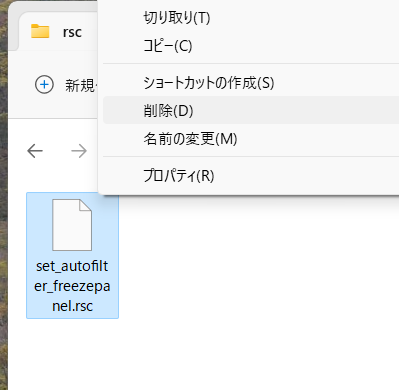
\includegraphics[width=0.3\textwidth,height=\textheight]{img/assoc_01.png}
\item
  拡張子が表示されていない場合は,エクスプローラの表示のオプションで,「登録されている拡張子は表示しない」のチェックを外して(チェックしないで),「OK」を選択してから,名前を変更する.\\
  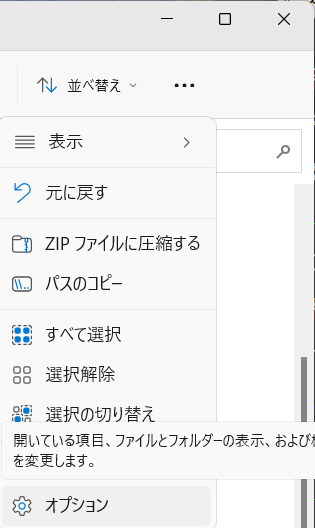
\includegraphics[width=0.4\textwidth,height=\textheight]{img/assoc_00_01.png}
  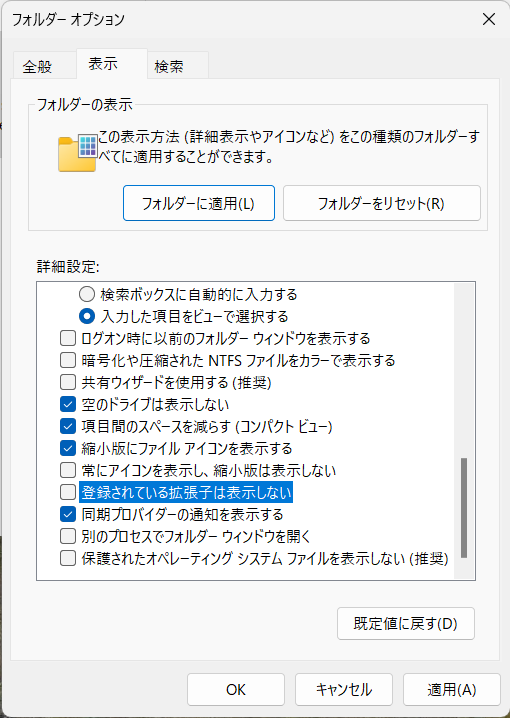
\includegraphics[width=0.4\textwidth,height=\textheight]{img/assoc_00_02.png}
\item
  ファイルを右クリックして,「プロパティ」を選択.\\
  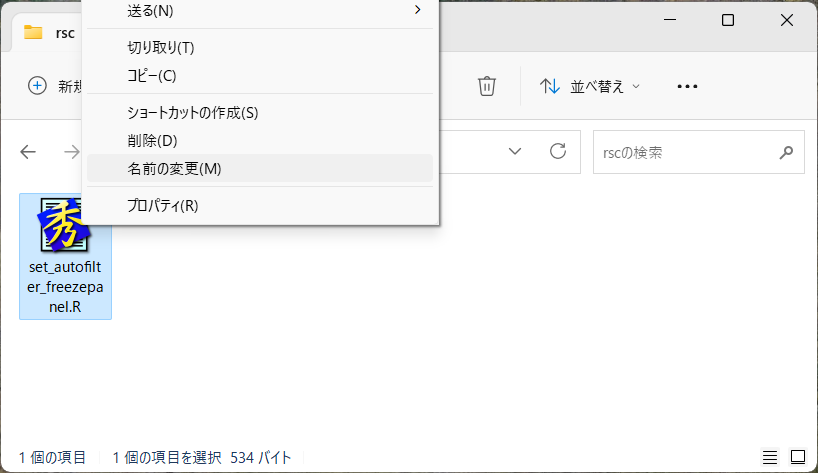
\includegraphics[width=0.3\textwidth,height=\textheight]{img/assoc_02.png}
\item
  「全般」タブのやや上にあるプログラムの「変更」を選択.\\
  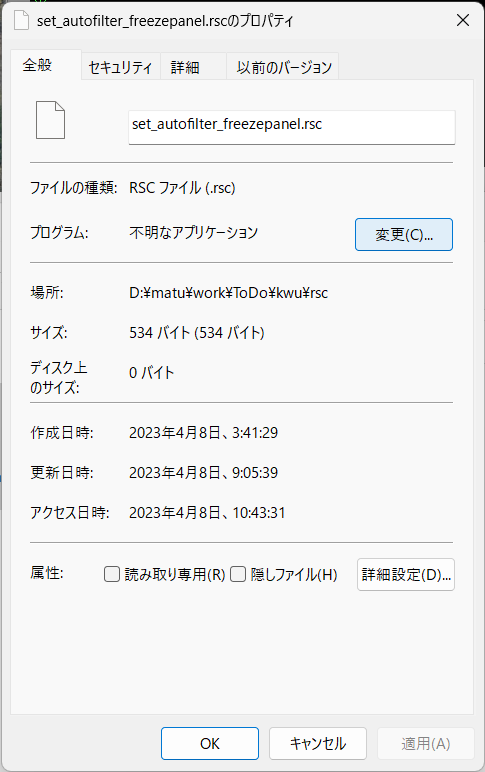
\includegraphics[width=0.5\textwidth,height=\textheight]{img/assoc_03.png}
\item
  「PCでアプリを選択する」をクリック.\\
  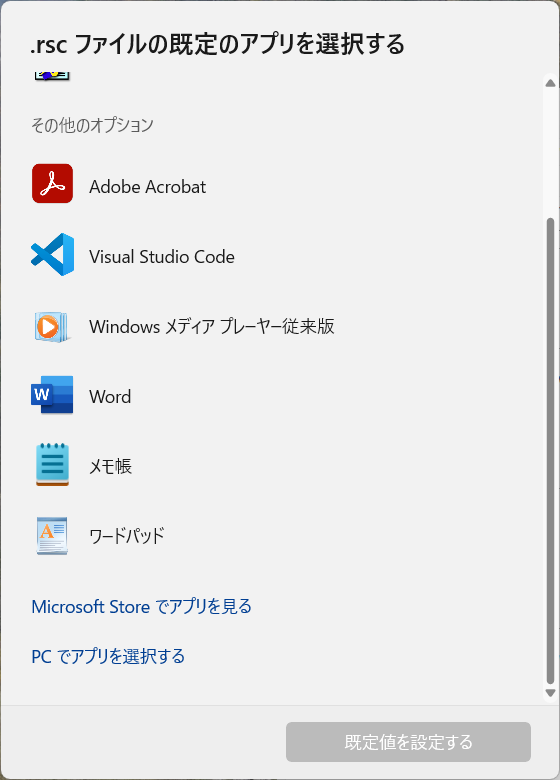
\includegraphics[width=0.5\textwidth,height=\textheight]{img/assoc_04.png}
\item
  ファイル選択画面で,Rをインストールしたフォルダまで辿っていき(「c:\textbackslash Program files\textbackslash R\textbackslash R-4.2.3\textbackslash bin\textbackslash x64」など),「Rscript.exe」を選択する.\\
  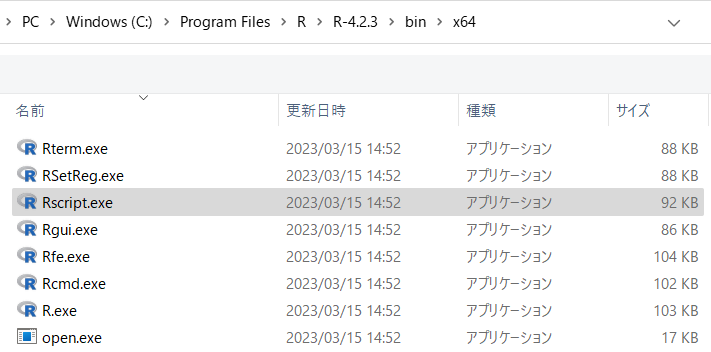
\includegraphics[width=0.5\textwidth,height=\textheight]{img/assoc_05.png}
\item
  「.rscファイルの既定のアプリを選択する」で「R for windows front-end」が表示されるので,「既定値を設定する」を選択.\\
  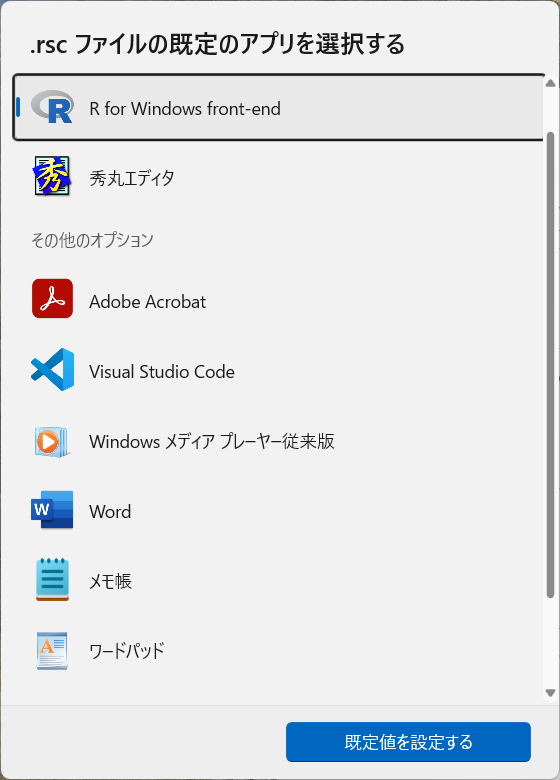
\includegraphics[width=0.5\textwidth,height=\textheight]{img/assoc_06.png}
\item
  全般タブのプログラムが「R for windows front-end」になっていることを確認して.「OK」を選択.\\
  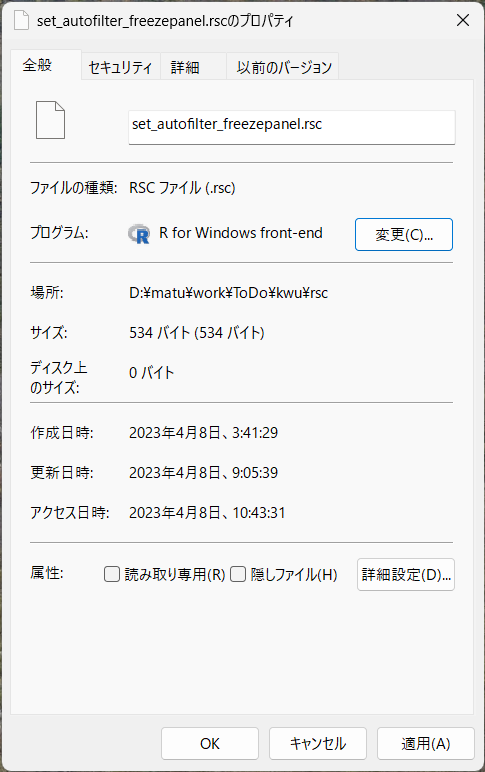
\includegraphics[width=0.5\textwidth,height=\textheight]{img/assoc_07.png}
\item
  ファイルのアイコンがRのアイコンになっていたらOK.\\
  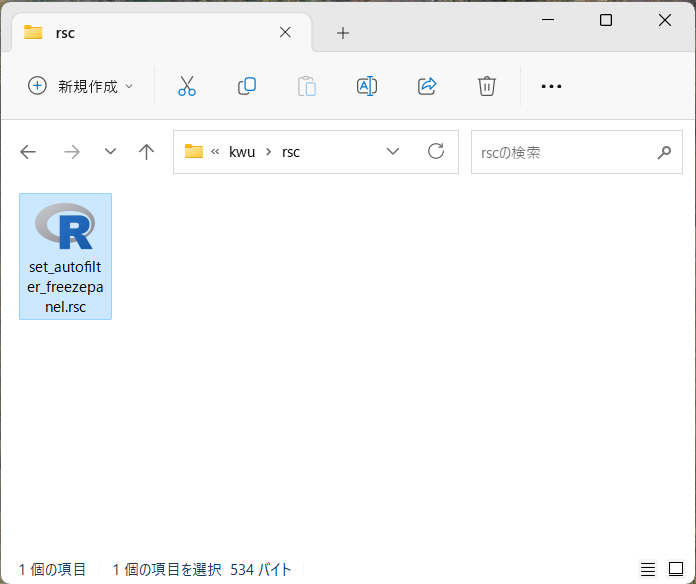
\includegraphics[width=0.3\textwidth,height=\textheight]{img/assoc_08.png}
\end{enumerate}

ダブルクリックすると,ファイルの内容が実行される(はず).

\hypertarget{ggplot2}{%
\section{ggplot2の勧め}\label{ggplot2}}

\hypertarget{rux306eux4f5cux56f3ux74b0ux5883ux306eux6982ux8981}{%
\subsection{Rの作図環境の概要}\label{rux306eux4f5cux56f3ux74b0ux5883ux306eux6982ux8981}}

\begin{itemize}
\tightlist
\item
  base(graphics)
\item
  lattice
\item
  grid
\item
  ggplot2
\end{itemize}

\hypertarget{ggplot2ux3068ux306f}{%
\subsection{ggplot2とは}\label{ggplot2ux3068ux306f}}

ggplot2は,tidy dataにしておけば,使いやすい

\hypertarget{ggplot2ux306eux5229ux70b9}{%
\subsection{ggplot2の利点}\label{ggplot2ux306eux5229ux70b9}}

1つのデータをもとに,ちょっとの変更で棒グラフ,散布図,などなど各種のplotが可能
図が綺麗で,テーマの変更も簡単
facetによるグループ分けも便利

magrittrとの相性も良い.
特にファイル名を設定するときの\texttt{\%\$\%}や\texttt{\%T\%}など

ggplot2をサポートするライブラリも豊富

凡例の自動的な位置決めや配置など
ggpubrなども

\hypertarget{ggplot2ux306eux57faux672c}{%
\subsection{ggplot2の基本}\label{ggplot2ux306eux57faux672c}}

irisを例にするが,できれば,veganとかdaveのデータを使う
tidy dataへの変換が必要
コードのみか,詳しくは松村や比嘉の解説を参考に

gather()とspread()はpivot\_longer()とpivot\_wider()になって使いやすくなった.
Hadley自身も使い方を混乱していたらしい

aesthetics

geom\_point()
geom\_bar()
aes()
colour
group
size

\hypertarget{facetux3092ux4f7fux304aux3046}{%
\subsection{facetを使おう}\label{facetux3092ux4f7fux304aux3046}}

forループやsubset,あるいはdplyr::filterを使っていたものが,一気にできて便利
コードも簡単で見やすい
コードの転用が簡単

group VS facet

\hypertarget{ggsave}{%
\subsection{ggsave}\label{ggsave}}

\begin{itemize}
\item
  pngとPDF\\
  PDFで日本語文字が化ける場合は,pngを使う
\item
  指定しないと,直前のプロット
\end{itemize}

\hypertarget{ux6587ux5b57ux5316ux3051ux3078ux306eux5bfeux51e6windows}{%
\subsection{文字化けへの対処(windows)}\label{ux6587ux5b57ux5316ux3051ux3078ux306eux5bfeux51e6windows}}

-cario?

\hypertarget{themeux3092ux5c11ux3057ux3060ux3051ux8aacux660e}{%
\subsection{themeを少しだけ説明}\label{themeux3092ux5c11ux3057ux3060ux3051ux8aacux660e}}

\begin{itemize}
\tightlist
\item
  デフォルト\\
\item
  theme\_bw()
\end{itemize}

\hypertarget{shiny}{%
\subsection{shiny}\label{shiny}}

Rだけでウェブアプリが作れる
reactiveの考え方を覚える必要あり

\hypertarget{ux53c2ux8003ux66f8}{%
\subsection{参考書}\label{ux53c2ux8003ux66f8}}

\begin{itemize}
\tightlist
\item
  ggplot2
\item
  ggplot2のレシピ
\item
  unwin GDA
\item
  チートシート
\end{itemize}

\hypertarget{magrittr}{%
\section{magrritrの勧め}\label{magrittr}}

\hypertarget{tidyverseux3068magrittr}{%
\subsection{tidyverseとmagrittr}\label{tidyverseux3068magrittr}}

tidyverseは,Rでのデータ解析には欠かせないものになっている.
そこで,Rを起動時にtidyverseを読み込む人は多いだろう.
なお,tidyverseは1つのライブラリではなく,複数のライブラリからなる.

\begin{Shaded}
\begin{Highlighting}[]
\FunctionTok{library}\NormalTok{(tidyverse)}
\end{Highlighting}
\end{Shaded}

これらのライブラリの多く(forcats,tibble,stringr,dplyr,tidyr,purrr)で,\texttt{\%\textgreater{}\%} (パイプ)を使うことができる.
私は\texttt{\%\textgreater{}\%}がtidyverse独自のものだと勘違いをしていた.
しかし,\texttt{\%\textgreater{}\%}はもとはライブラリmagrittrの関数であり,そこからインポートされている.
そのため,tidyverseを読み込むと使うことができる.
\texttt{\%\textgreater{}\%}は,慣れるまでは何が便利なのか分からないが,慣れると欠かせなくなる.
さらに使っていると,癖なってしまって無駄にパイプを繋ぐこともある.
長過ぎるパイプは良くないのは当然であるものの,適度に使うとRでのプログラミングは非常に楽になる.

tidyverseの関数では,引数とするオブジェクトが統一されている.
具体的には,第1引数のオブジェクトがデータフレームやtibbleになっていることが多い.
そのため,パイプと相性が特に良い.

\hypertarget{ux3068ux305dux306eux4ef2ux9593}{%
\subsection{\texorpdfstring{\texttt{\%\textgreater{}\%}とその仲間}{\%\textgreater\%とその仲間}}\label{ux3068ux305dux306eux4ef2ux9593}}

\texttt{\%\textgreater{}\%}の仲間としては,以下の関数もある.

\begin{itemize}
\tightlist
\item
  \texttt{\%\textless{}\textgreater{}\%}
\item
  \texttt{\%T\textgreater{}\%}
\item
  \texttt{\%\$\%}
\end{itemize}

これらの関数は,tidyverseには含まれていないため,使用するにはmagrittrを読み込む必要がある.

\begin{Shaded}
\begin{Highlighting}[]
\FunctionTok{library}\NormalTok{(magrittr)}
\end{Highlighting}
\end{Shaded}

\begin{verbatim}
## 
## Attaching package: 'magrittr'
\end{verbatim}

\begin{verbatim}
## The following object is masked from 'package:purrr':
## 
##     set_names
\end{verbatim}

\begin{verbatim}
## The following object is masked from 'package:tidyr':
## 
##     extract
\end{verbatim}

\hypertarget{section}{%
\subsection{\texorpdfstring{\texttt{\%\textless{}\textgreater{}\%}}{\%\textless\textgreater\%}}\label{section}}

\hypertarget{ux4f7fux3044ux65b9}{%
\subsubsection{使い方}\label{ux4f7fux3044ux65b9}}

\texttt{\%\textless{}\textgreater{}\%}は,パイプを使って処理した内容を,最初のオブジェクトに再度代入するときに使う.
ほんの少しだけ,コードを短くできる.

\begin{Shaded}
\begin{Highlighting}[]
\NormalTok{mpg }\CommentTok{\# 燃費データ}
\end{Highlighting}
\end{Shaded}

\begin{verbatim}
## # A tibble: 234 x 11
##    manufacturer model      displ  year   cyl trans drv     cty   hwy fl    class
##    <chr>        <chr>      <dbl> <int> <int> <chr> <chr> <int> <int> <chr> <chr>
##  1 audi         a4           1.8  1999     4 auto~ f        18    29 p     comp~
##  2 audi         a4           1.8  1999     4 manu~ f        21    29 p     comp~
##  3 audi         a4           2    2008     4 manu~ f        20    31 p     comp~
##  4 audi         a4           2    2008     4 auto~ f        21    30 p     comp~
##  5 audi         a4           2.8  1999     6 auto~ f        16    26 p     comp~
##  6 audi         a4           2.8  1999     6 manu~ f        18    26 p     comp~
##  7 audi         a4           3.1  2008     6 auto~ f        18    27 p     comp~
##  8 audi         a4 quattro   1.8  1999     4 manu~ 4        18    26 p     comp~
##  9 audi         a4 quattro   1.8  1999     4 auto~ 4        16    25 p     comp~
## 10 audi         a4 quattro   2    2008     4 manu~ 4        20    28 p     comp~
## # ... with 224 more rows
\end{verbatim}

\begin{Shaded}
\begin{Highlighting}[]
\NormalTok{tmp }\OtherTok{\textless{}{-}}\NormalTok{ mpg}
\NormalTok{tmp }\OtherTok{\textless{}{-}}
\NormalTok{  tmp }\SpecialCharTok{\%\textgreater{}\%}
\NormalTok{  dplyr}\SpecialCharTok{::}\FunctionTok{filter}\NormalTok{(year}\SpecialCharTok{==}\DecValTok{1999}\NormalTok{) }\SpecialCharTok{\%\textgreater{}\%}
\NormalTok{  tidyr}\SpecialCharTok{::}\FunctionTok{separate}\NormalTok{(trans, }\AttributeTok{into=}\FunctionTok{c}\NormalTok{(}\StringTok{"trans1"}\NormalTok{, }\StringTok{"trans2"}\NormalTok{, }\ConstantTok{NA}\NormalTok{)) }\SpecialCharTok{\%\textgreater{}\%}
  \FunctionTok{print}\NormalTok{()}
\end{Highlighting}
\end{Shaded}

\begin{verbatim}
## # A tibble: 117 x 12
##    manufac~1 model displ  year   cyl trans1 trans2 drv     cty   hwy fl    class
##    <chr>     <chr> <dbl> <int> <int> <chr>  <chr>  <chr> <int> <int> <chr> <chr>
##  1 audi      a4      1.8  1999     4 auto   l5     f        18    29 p     comp~
##  2 audi      a4      1.8  1999     4 manual m5     f        21    29 p     comp~
##  3 audi      a4      2.8  1999     6 auto   l5     f        16    26 p     comp~
##  4 audi      a4      2.8  1999     6 manual m5     f        18    26 p     comp~
##  5 audi      a4 q~   1.8  1999     4 manual m5     4        18    26 p     comp~
##  6 audi      a4 q~   1.8  1999     4 auto   l5     4        16    25 p     comp~
##  7 audi      a4 q~   2.8  1999     6 auto   l5     4        15    25 p     comp~
##  8 audi      a4 q~   2.8  1999     6 manual m5     4        17    25 p     comp~
##  9 audi      a6 q~   2.8  1999     6 auto   l5     4        15    24 p     mids~
## 10 chevrolet c150~   5.7  1999     8 auto   l4     r        13    17 r     suv  
## # ... with 107 more rows, and abbreviated variable name 1: manufacturer
\end{verbatim}

\begin{Shaded}
\begin{Highlighting}[]
\NormalTok{tmp }\OtherTok{\textless{}{-}}\NormalTok{ mpg}
\NormalTok{tmp }\SpecialCharTok{\%\textless{}\textgreater{}\%}
\NormalTok{  dplyr}\SpecialCharTok{::}\FunctionTok{filter}\NormalTok{(year}\SpecialCharTok{==}\DecValTok{1999}\NormalTok{) }\SpecialCharTok{\%\textgreater{}\%}
\NormalTok{  tidyr}\SpecialCharTok{::}\FunctionTok{separate}\NormalTok{(trans, }\AttributeTok{into=}\FunctionTok{c}\NormalTok{(}\StringTok{"trans1"}\NormalTok{, }\StringTok{"trans2"}\NormalTok{, }\ConstantTok{NA}\NormalTok{)) }\SpecialCharTok{\%\textgreater{}\%}
  \FunctionTok{print}\NormalTok{()}
\end{Highlighting}
\end{Shaded}

\begin{verbatim}
## # A tibble: 117 x 12
##    manufac~1 model displ  year   cyl trans1 trans2 drv     cty   hwy fl    class
##    <chr>     <chr> <dbl> <int> <int> <chr>  <chr>  <chr> <int> <int> <chr> <chr>
##  1 audi      a4      1.8  1999     4 auto   l5     f        18    29 p     comp~
##  2 audi      a4      1.8  1999     4 manual m5     f        21    29 p     comp~
##  3 audi      a4      2.8  1999     6 auto   l5     f        16    26 p     comp~
##  4 audi      a4      2.8  1999     6 manual m5     f        18    26 p     comp~
##  5 audi      a4 q~   1.8  1999     4 manual m5     4        18    26 p     comp~
##  6 audi      a4 q~   1.8  1999     4 auto   l5     4        16    25 p     comp~
##  7 audi      a4 q~   2.8  1999     6 auto   l5     4        15    25 p     comp~
##  8 audi      a4 q~   2.8  1999     6 manual m5     4        17    25 p     comp~
##  9 audi      a6 q~   2.8  1999     6 auto   l5     4        15    24 p     mids~
## 10 chevrolet c150~   5.7  1999     8 auto   l4     r        13    17 r     suv  
## # ... with 107 more rows, and abbreviated variable name 1: manufacturer
\end{verbatim}

\hypertarget{ux6ce8ux610fux70b9}{%
\subsubsection{注意点}\label{ux6ce8ux610fux70b9}}

試行錯誤でコードを書いている途中は,あまり使わないほうが良いだろう.
もとのオブジェクトが置き換わるので,処理結果が求めるものでないときに,もとに戻れないためである.

\hypertarget{t}{%
\subsection{\texorpdfstring{\texttt{\%T\textgreater{}\%}}{\%T\textgreater\%}}\label{t}}

\hypertarget{ux4f7fux3044ux65b9-1}{%
\subsubsection{使い方}\label{ux4f7fux3044ux65b9-1}}

処理途中に分岐をして別の処理をさせたいときに使う.
ちょっとだけ処理して,変数に保存するとき
imapと組み合わせると便利かも
画像を保存するファイル名の設定とか

\begin{Shaded}
\begin{Highlighting}[]
\NormalTok{mpg }\CommentTok{\# 燃費データ}
\end{Highlighting}
\end{Shaded}

\begin{verbatim}
## # A tibble: 234 x 11
##    manufacturer model      displ  year   cyl trans drv     cty   hwy fl    class
##    <chr>        <chr>      <dbl> <int> <int> <chr> <chr> <int> <int> <chr> <chr>
##  1 audi         a4           1.8  1999     4 auto~ f        18    29 p     comp~
##  2 audi         a4           1.8  1999     4 manu~ f        21    29 p     comp~
##  3 audi         a4           2    2008     4 manu~ f        20    31 p     comp~
##  4 audi         a4           2    2008     4 auto~ f        21    30 p     comp~
##  5 audi         a4           2.8  1999     6 auto~ f        16    26 p     comp~
##  6 audi         a4           2.8  1999     6 manu~ f        18    26 p     comp~
##  7 audi         a4           3.1  2008     6 auto~ f        18    27 p     comp~
##  8 audi         a4 quattro   1.8  1999     4 manu~ 4        18    26 p     comp~
##  9 audi         a4 quattro   1.8  1999     4 auto~ 4        16    25 p     comp~
## 10 audi         a4 quattro   2    2008     4 manu~ 4        20    28 p     comp~
## # ... with 224 more rows
\end{verbatim}

\hypertarget{ux6ce8ux610fux70b9-1}{%
\subsubsection{注意点}\label{ux6ce8ux610fux70b9-1}}

分岐途中の結果をオブジェクトに代入するときには,\texttt{\textless{}-}ではなく,\texttt{\textless{}\textless{}-}を使用する.
明示的に「.」を使う
複数処理があれば,「\{\}」で囲う
処理終了後に「\%\textgreater\%」が必要
例のコードを示す

\begin{Shaded}
\begin{Highlighting}[]
\CommentTok{\#  mpg \%T\textgreater{}\%}
\CommentTok{\#    \{}
\CommentTok{\#      tmp \textless{}\textless{}{-} dplyr::select(., ) }
\CommentTok{\#    \} \%\textgreater{}\%}
\end{Highlighting}
\end{Shaded}

\hypertarget{section-1}{%
\subsection{\texorpdfstring{\texttt{\%\$\%}}{\%\$\%}}\label{section-1}}

\hypertarget{ux4f7fux3044ux65b9-2}{%
\subsubsection{使い方}\label{ux4f7fux3044ux65b9-2}}

\begin{Shaded}
\begin{Highlighting}[]
\NormalTok{mpg }\SpecialCharTok{\%\textgreater{}\%}
\NormalTok{  .}\SpecialCharTok{$}\NormalTok{manufacturer}
\end{Highlighting}
\end{Shaded}

\begin{verbatim}
##   [1] "audi"       "audi"       "audi"       "audi"       "audi"      
##   [6] "audi"       "audi"       "audi"       "audi"       "audi"      
##  [11] "audi"       "audi"       "audi"       "audi"       "audi"      
##  [16] "audi"       "audi"       "audi"       "chevrolet"  "chevrolet" 
##  [21] "chevrolet"  "chevrolet"  "chevrolet"  "chevrolet"  "chevrolet" 
##  [26] "chevrolet"  "chevrolet"  "chevrolet"  "chevrolet"  "chevrolet" 
##  [31] "chevrolet"  "chevrolet"  "chevrolet"  "chevrolet"  "chevrolet" 
##  [36] "chevrolet"  "chevrolet"  "dodge"      "dodge"      "dodge"     
##  [41] "dodge"      "dodge"      "dodge"      "dodge"      "dodge"     
##  [46] "dodge"      "dodge"      "dodge"      "dodge"      "dodge"     
##  [51] "dodge"      "dodge"      "dodge"      "dodge"      "dodge"     
##  [56] "dodge"      "dodge"      "dodge"      "dodge"      "dodge"     
##  [61] "dodge"      "dodge"      "dodge"      "dodge"      "dodge"     
##  [66] "dodge"      "dodge"      "dodge"      "dodge"      "dodge"     
##  [71] "dodge"      "dodge"      "dodge"      "dodge"      "ford"      
##  [76] "ford"       "ford"       "ford"       "ford"       "ford"      
##  [81] "ford"       "ford"       "ford"       "ford"       "ford"      
##  [86] "ford"       "ford"       "ford"       "ford"       "ford"      
##  [91] "ford"       "ford"       "ford"       "ford"       "ford"      
##  [96] "ford"       "ford"       "ford"       "ford"       "honda"     
## [101] "honda"      "honda"      "honda"      "honda"      "honda"     
## [106] "honda"      "honda"      "honda"      "hyundai"    "hyundai"   
## [111] "hyundai"    "hyundai"    "hyundai"    "hyundai"    "hyundai"   
## [116] "hyundai"    "hyundai"    "hyundai"    "hyundai"    "hyundai"   
## [121] "hyundai"    "hyundai"    "jeep"       "jeep"       "jeep"      
## [126] "jeep"       "jeep"       "jeep"       "jeep"       "jeep"      
## [131] "land rover" "land rover" "land rover" "land rover" "lincoln"   
## [136] "lincoln"    "lincoln"    "mercury"    "mercury"    "mercury"   
## [141] "mercury"    "nissan"     "nissan"     "nissan"     "nissan"    
## [146] "nissan"     "nissan"     "nissan"     "nissan"     "nissan"    
## [151] "nissan"     "nissan"     "nissan"     "nissan"     "pontiac"   
## [156] "pontiac"    "pontiac"    "pontiac"    "pontiac"    "subaru"    
## [161] "subaru"     "subaru"     "subaru"     "subaru"     "subaru"    
## [166] "subaru"     "subaru"     "subaru"     "subaru"     "subaru"    
## [171] "subaru"     "subaru"     "subaru"     "toyota"     "toyota"    
## [176] "toyota"     "toyota"     "toyota"     "toyota"     "toyota"    
## [181] "toyota"     "toyota"     "toyota"     "toyota"     "toyota"    
## [186] "toyota"     "toyota"     "toyota"     "toyota"     "toyota"    
## [191] "toyota"     "toyota"     "toyota"     "toyota"     "toyota"    
## [196] "toyota"     "toyota"     "toyota"     "toyota"     "toyota"    
## [201] "toyota"     "toyota"     "toyota"     "toyota"     "toyota"    
## [206] "toyota"     "toyota"     "volkswagen" "volkswagen" "volkswagen"
## [211] "volkswagen" "volkswagen" "volkswagen" "volkswagen" "volkswagen"
## [216] "volkswagen" "volkswagen" "volkswagen" "volkswagen" "volkswagen"
## [221] "volkswagen" "volkswagen" "volkswagen" "volkswagen" "volkswagen"
## [226] "volkswagen" "volkswagen" "volkswagen" "volkswagen" "volkswagen"
## [231] "volkswagen" "volkswagen" "volkswagen" "volkswagen"
\end{verbatim}

\begin{Shaded}
\begin{Highlighting}[]
\NormalTok{mpg }\SpecialCharTok{\%$\%}
\NormalTok{  manufacturer}
\end{Highlighting}
\end{Shaded}

\begin{verbatim}
##   [1] "audi"       "audi"       "audi"       "audi"       "audi"      
##   [6] "audi"       "audi"       "audi"       "audi"       "audi"      
##  [11] "audi"       "audi"       "audi"       "audi"       "audi"      
##  [16] "audi"       "audi"       "audi"       "chevrolet"  "chevrolet" 
##  [21] "chevrolet"  "chevrolet"  "chevrolet"  "chevrolet"  "chevrolet" 
##  [26] "chevrolet"  "chevrolet"  "chevrolet"  "chevrolet"  "chevrolet" 
##  [31] "chevrolet"  "chevrolet"  "chevrolet"  "chevrolet"  "chevrolet" 
##  [36] "chevrolet"  "chevrolet"  "dodge"      "dodge"      "dodge"     
##  [41] "dodge"      "dodge"      "dodge"      "dodge"      "dodge"     
##  [46] "dodge"      "dodge"      "dodge"      "dodge"      "dodge"     
##  [51] "dodge"      "dodge"      "dodge"      "dodge"      "dodge"     
##  [56] "dodge"      "dodge"      "dodge"      "dodge"      "dodge"     
##  [61] "dodge"      "dodge"      "dodge"      "dodge"      "dodge"     
##  [66] "dodge"      "dodge"      "dodge"      "dodge"      "dodge"     
##  [71] "dodge"      "dodge"      "dodge"      "dodge"      "ford"      
##  [76] "ford"       "ford"       "ford"       "ford"       "ford"      
##  [81] "ford"       "ford"       "ford"       "ford"       "ford"      
##  [86] "ford"       "ford"       "ford"       "ford"       "ford"      
##  [91] "ford"       "ford"       "ford"       "ford"       "ford"      
##  [96] "ford"       "ford"       "ford"       "ford"       "honda"     
## [101] "honda"      "honda"      "honda"      "honda"      "honda"     
## [106] "honda"      "honda"      "honda"      "hyundai"    "hyundai"   
## [111] "hyundai"    "hyundai"    "hyundai"    "hyundai"    "hyundai"   
## [116] "hyundai"    "hyundai"    "hyundai"    "hyundai"    "hyundai"   
## [121] "hyundai"    "hyundai"    "jeep"       "jeep"       "jeep"      
## [126] "jeep"       "jeep"       "jeep"       "jeep"       "jeep"      
## [131] "land rover" "land rover" "land rover" "land rover" "lincoln"   
## [136] "lincoln"    "lincoln"    "mercury"    "mercury"    "mercury"   
## [141] "mercury"    "nissan"     "nissan"     "nissan"     "nissan"    
## [146] "nissan"     "nissan"     "nissan"     "nissan"     "nissan"    
## [151] "nissan"     "nissan"     "nissan"     "nissan"     "pontiac"   
## [156] "pontiac"    "pontiac"    "pontiac"    "pontiac"    "subaru"    
## [161] "subaru"     "subaru"     "subaru"     "subaru"     "subaru"    
## [166] "subaru"     "subaru"     "subaru"     "subaru"     "subaru"    
## [171] "subaru"     "subaru"     "subaru"     "toyota"     "toyota"    
## [176] "toyota"     "toyota"     "toyota"     "toyota"     "toyota"    
## [181] "toyota"     "toyota"     "toyota"     "toyota"     "toyota"    
## [186] "toyota"     "toyota"     "toyota"     "toyota"     "toyota"    
## [191] "toyota"     "toyota"     "toyota"     "toyota"     "toyota"    
## [196] "toyota"     "toyota"     "toyota"     "toyota"     "toyota"    
## [201] "toyota"     "toyota"     "toyota"     "toyota"     "toyota"    
## [206] "toyota"     "toyota"     "volkswagen" "volkswagen" "volkswagen"
## [211] "volkswagen" "volkswagen" "volkswagen" "volkswagen" "volkswagen"
## [216] "volkswagen" "volkswagen" "volkswagen" "volkswagen" "volkswagen"
## [221] "volkswagen" "volkswagen" "volkswagen" "volkswagen" "volkswagen"
## [226] "volkswagen" "volkswagen" "volkswagen" "volkswagen" "volkswagen"
## [231] "volkswagen" "volkswagen" "volkswagen" "volkswagen"
\end{verbatim}

\hypertarget{ux6ce8ux610fux70b9-2}{%
\subsubsection{注意点}\label{ux6ce8ux610fux70b9-2}}

\hypertarget{rvest}{%
\section{rvestでスクレイピング}\label{rvest}}

\hypertarget{ux30b9ux30afux30ecux30a4ux30d4ux30f3ux30b0}{%
\subsection{スクレイピング}\label{ux30b9ux30afux30ecux30a4ux30d4ux30f3ux30b0}}

ここでのスクレイピングとは,ウェブスクレイピングの省略のことで,ウェブサイトにある情報を収集することである.
ウェブサイトから植生調査データを収集することはほとんどないものの,関連データの収集は可能である.
例えば,気象庁のページから気象データが収集可能である.
もちろん,気象データは手動でも収集可能ではあるが,多大な手間と長い時間が必要である.
研究に必要なデータを自動で取得できれば,手間と時間の節約が可能である.

そこで,本稿ではウェブでの情報収集の方法を紹介することを目的とする.
世界の各地点の気象データをプロット
情報収集にはRのパッケージであるrvestを用いる.
rvestを用いて気象庁のページから世界の気象データを入手して,気候ダイアグラムを描画する.

Rのパッケージ作成では,rvestを用いて作成した関数と収集したデータをまとめたパッケージの作成方法を紹介する.
著者自身,他人のためにパッケージをつくることは考えておらず,基本的には自分の研究や作業のための関数をまとめることを目的としてパッケージをいくつか作成した.
作成したら,ついでに他人にも使ってもらえれば嬉しいという程度である.

過去に作成した関数は,しばらくすると関数の引数や返り値がどのようなものであったのか忘れてしまいがちである.
パッケージをつくる(特にCRANに登録する)には,引数,返り値,使用例などをまとめる必要がある.
きっちりまとめなくても良いのではあるが,決まった形式の方がむしろまとめやすい.
また,RStudioとusethis, testthat, devtoolsなどのパッケージを使ってパッケージ開発すると,各種チェックやテストが可能である.
各種チェックやテストでたくさんのエラーを見ると,チェックやテストは正直なところ煩わしいと感じる.
特に,パケージ開発に慣れていないと特にそうである.
しかし,チェックやテストをすることで,関数の完成度を確実に高めることができるため,パッケージとしてまとめる利点である.

\hypertarget{rvest-ux3068-rselenium}{%
\subsection{rvest と RSelenium}\label{rvest-ux3068-rselenium}}

スクレイピングをするために使われる主なRのパッケージとしては,rvestとRSeleniumがある.
rvestは,静的なサイトを対象とするときに役立つ.
つまり,URLを指定すれば対象のサイトのページが決まるときである.
気象庁での気象データを提供しているページがこれに当たる.
一方,RSeleniumは動的なサイトを対象とするときに役立つ.
例えば,テキストボックスへのデータ入力やプルダウンメニューの選択あるいはその後のマウス操作でページが遷移する場合である.
このような動的なサイトでは,Seleniumだけでなく,Javascriptを部分的に用いるのも効果的である.
なお,rvestでもユーザ名とパスワードを用いた一般的なログインは可能である.
また,politeパッケージと組み合わせることである程度の動的なサイトのスクレイピングは可能である.

\hypertarget{rvestux306eux3067ux304dux308bux3053ux3068}{%
\subsection{rvestのできること}\label{rvestux306eux3067ux304dux308bux3053ux3068}}

\begin{itemize}
\tightlist
\item
  HTMLの取得\\
\item
  DOMの取得: id, class, tagNameなどを用いる\\
\item
  tableの取得

  \begin{itemize}
  \tightlist
  \item
    HTML内の取得したいデータはtableにあることが多いため,非常に便利
    そもそも,tableでないデータを取得するのは非常に不便
  \end{itemize}
\item
  リンクの取得\\
  ページ遷移に使用する\\
\item
  stringrと組み合わせて使うと良い\\
\item
  文字コードの変換にはstringiを用いる\\
\item
  tidyverseやmagrittrとの合せ技が便利\\
\item
  Formの入力・選択
  radioボタンはちょっと工夫が必要
  moranajp::html\_radio\_set()
  無理やりな感じではあるが,同一名称のradioボタンを全て同じ値に変更する
  本来なら,不要なradioボタンのフォームを削除
  可能だが,インデクスがずれるので結構厄介
  politeパッケージとの連携
\end{itemize}

\hypertarget{ux6e96ux5099}{%
\subsection{準備}\label{ux6e96ux5099}}

\begin{Shaded}
\begin{Highlighting}[]
  \CommentTok{\# install.packages("rvest")}
  \CommentTok{\# library(rvest)}
\end{Highlighting}
\end{Shaded}

\hypertarget{htmlux306eux53d6ux5f97}{%
\subsection{HTMLの取得}\label{htmlux306eux53d6ux5f97}}

\hypertarget{ux4f7fux3044ux65b9-3}{%
\subsubsection{使い方}\label{ux4f7fux3044ux65b9-3}}

\hypertarget{ux6ce8ux610fux70b9-3}{%
\subsubsection{注意点}\label{ux6ce8ux610fux70b9-3}}

\hypertarget{domux306eux53d6ux5f97}{%
\subsection{DOMの取得}\label{domux306eux53d6ux5f97}}

\hypertarget{ux4f7fux3044ux65b9-4}{%
\subsubsection{使い方}\label{ux4f7fux3044ux65b9-4}}

\hypertarget{ux6ce8ux610fux70b9-4}{%
\subsubsection{注意点}\label{ux6ce8ux610fux70b9-4}}

\hypertarget{rselenium}{%
\section{Rselenium}\label{rselenium}}

Seleniumは,ブラウザを使って動的に巡回しつつ,スクレイピングをするのに適している.

JavascriptやPHPなどを使って,動的に作成されるサイトでは,URLだけではページを特定することはできない.
そのため,rvestだけではデータを取得するのが困難である.

\hypertarget{ux6e96ux5099-1}{%
\subsection{準備}\label{ux6e96ux5099-1}}

\begin{itemize}
\tightlist
\item
  RSelenium: CRANからインストール\\
\item
  Selenium: 本家サイトからインストール

  \begin{itemize}
  \tightlist
  \item
    注意: ver3.xxx をインストールする\\
    ver4.0 以上はRSeleniumuが対応していない(Pythonなら可)\\
  \end{itemize}
\item
  ChromeDriver

  \begin{itemize}
  \tightlist
  \item
    注意: 自身の利用しているブラウザのドライバが必要(バージョンも合致する必要あり)
    GoogleChromeは自動的にupdateされるので,バージョンをよく確認する
    通常は,安定版の最新版で大丈夫である
  \item
    Seleniumと同じフォルダに保存する
  \end{itemize}
\end{itemize}

\hypertarget{ux30d6ux30e9ux30a6ux30b6ux306eux81eaux52d5ux5316}{%
\subsection{ブラウザの自動化}\label{ux30d6ux30e9ux30a6ux30b6ux306eux81eaux52d5ux5316}}

\hypertarget{section-2}{%
\subsection{}\label{section-2}}

\hypertarget{ux4f7fux3044ux65b9-5}{%
\subsubsection{使い方}\label{ux4f7fux3044ux65b9-5}}

\hypertarget{ux6ce8ux610fux70b9-5}{%
\subsubsection{注意点}\label{ux6ce8ux610fux70b9-5}}

\hypertarget{ux8981ux7d20ux306eux53d6ux5f97}{%
\subsection{要素の取得}\label{ux8981ux7d20ux306eux53d6ux5f97}}

idがわかるとき
document.getElementByID()

xpath
document.selectQueryAll(){[}{]}
動的にサイトが作られているときには,変化する可能性があるので注意

使用されているJavaScriptの関数がわかる
script \textless- ``\,''
rem\$excute(script)

例
BiSSの文字サイズの変更
主命リストの列数の変更

スクレイピングの実行時には,適切な時間間隔を空ける
- 通常は5秒以上を求めていることが多い

ページ遷移の命令を送信後,十分な間隔がないとHTMLの要素を取得しきれていないことがある
極端な場合,サーバーからの情報がほとんど何も送られていない,つまりページの内容がほとんど何もないことにある.
この状況は,通常のマウス操作では何も表示されていないところをクリックするのと同じ状態である.
サーバからの情報を待つ意味でも適度な間隔を空けるのが望ましい

動的なサイトの場合は,HTMLの構成中の可能性もある
ログイン等のページでも,遷移途中のことがある.

\hypertarget{ux305dux306eux4ed6}{%
\subsection{その他}\label{ux305dux306eux4ed6}}

\begin{itemize}
\tightlist
\item
  Rからシェルのコマンドを使う

  \begin{itemize}
  \tightlist
  \item
    pngからPDFへ変換\\
  \item
    ファイルの移動\\
  \item
    Seleniumuの起動・終了\\
  \item
    MeCabやGINZAの実行
  \end{itemize}
\end{itemize}

\hypertarget{shell}{%
\section{shell}\label{shell}}

\begin{itemize}
\tightlist
\item
  Rからシェルのコマンドを使う

  \begin{itemize}
  \tightlist
  \item
    ファイルの移動\\
  \item
    PDFファイルの結合\\
  \item
    pngからPDFへ変換
  \end{itemize}
\end{itemize}

手作業でも良いが,ファイル数が多かったり,作業回数が多かったりするなら,自動化するのが便利である.
例えば,ファイルの操作やちょっとしたCUIアプリをコマンドでの動作をRでやってしまおうという邪道中の邪道である.
上記の操作をする際は,LinuxやMacであればshellスクリプトとして,Windowsであればバッチファイルとしてコードを書くのが本来の方法である.
しかし,shellスクリプトやバッチファイルのコマンドを体系的に勉強したことはない(その意味ではRの勉強もかなり怪しい).
ウェブの情報をもとにしつつ,なんとなくコードを書いたことはある.
とはいえ変数の使い方などは特によくわからないので,ちょっとした操作にも時間がかかりそう.
そこで,慣れたRを使って雑多な操作をやっつけてしまおうと考えた.

以下のような操作を自動化する.
・複数のフォルダに入ったPDFファイルを1つのPDFに結合
・結合後のファイルを指定場所に移動
・元ファイルを削除

なお,以下は基本的にwindowsでの操作を前提としているが,LinuxやMacでも同じあるいは類似のコマンドで代用できる可能性が高い.
日本語文字が入っていると,操作に若干手間がかかることが多い.

dosコマンド
ls, dir
ファイル,ディレクトリの一覧を取得
move, copy, remove, rename
ファイルの移動,コピー,削除, リネーム
cd
ディレクトリの移動

Rの関数
shell(), system()
コマンドの実行
setwd()
ワーキングディレクトリの設定
ディレクトリ名にスペースや日本語が入っていて,cdコマンドがうまくいかないときは,こっちのほうが便利
paste0()
文字列の結合
stringrの関数
stringiの関数
多くの関数はstringrにラッパーがあるが,文字コードの変換などはstringiの関数が必要
日本語文字を使わなければ不要
ファイル名の命名規則を決めておき,お世話にならない方が幸せ
purrr::map()
for loopの代わり
\# ファイル名を取得する関数など

その他ツール
concatPDF
PDFの結合など(win10 OK,win11 NG)
\# ConcatPDF /outfile Merged.pdf File1.pdf File2.pdf File3.pdf

pdftk
PDFの結合など(win11 OK)
pdftk File1.pdf File2.pdf File3.pdf cat output Merged.pdf

ImageMagick
画像変換など

\hypertarget{ux6e96ux5099-2}{%
\subsection{準備}\label{ux6e96ux5099-2}}

\hypertarget{dbi}{%
\section{DBIでデータ取得}\label{dbi}}

\hypertarget{ux30c7ux30fcux30bfux30d9ux30fcux30b9ux3068ux306eux9023ux643a}{%
\subsection{データベースとの連携}\label{ux30c7ux30fcux30bfux30d9ux30fcux30b9ux3068ux306eux9023ux643a}}

リレーショナル・データベースと接続してデータを取得するためのパッケージには色々とある.

CRAN Task View: Databases with R には多くのパッケージが掲載されている.
\url{https://cran.r-project.org/web/views/Databases.html}

どれを使っても良いが,よく使われているのはDBIのようだ.
\url{https://cran.r-project.org/web/packages/DBI/index.html}

\hypertarget{dbiux3067ux3067ux304dux308bux3053ux3068}{%
\subsection{DBIでできること}\label{dbiux3067ux3067ux304dux308bux3053ux3068}}

\begin{itemize}
\tightlist
\item
  各種データベースとの接続\\
\item
  SQLによるデータ操作
\end{itemize}

SQLを使い慣れていれば,SQLで各種の操作をするのが良いだろう.
一方,Rでのデータフレームの操作に慣れていれば,取得したデータをRで操作するのが良い.
つまり,データ取得だけにDBIを利用して,その後はdplyrやtidyverseの各種パッケージの関数を駆使してデータを処理する.
さらに,その結果を図示したい場合は,ggplot2を使うと良い.

\hypertarget{ux6e96ux5099-3}{%
\subsection{準備}\label{ux6e96ux5099-3}}

\begin{Shaded}
\begin{Highlighting}[]
\FunctionTok{install.packages}\NormalTok{(}\StringTok{"DBI"}\NormalTok{)}
\FunctionTok{library}\NormalTok{(DBI)}
\end{Highlighting}
\end{Shaded}

\hypertarget{ux4f7fux3044ux65b9-6}{%
\subsection{使い方}\label{ux4f7fux3044ux65b9-6}}

詳細は以下を参照.

\url{https://cran.r-project.org/web/packages/DBI/vignettes/DBI-1.html}

\hypertarget{xlsx}{%
\section{xlsxでエクセル操作}\label{xlsx}}

xlsxパッケージを使うと,エクセルのファイルの読み込み・書き込みをはじめ,
オートフィルタの設定やウィンドウ枠の固定などの各種操作が可能である.

\hypertarget{ux30aaux30fcux30c8ux30d5ux30a3ux30ebux30bfux306eux8a2dux5b9aux3068ux30a6ux30a3ux30f3ux30c9ux30a6ux67a0ux306eux56faux5b9aux306eux81eaux52d5ux5316ux30b9ux30afux30eaux30d7ux30c8}{%
\subsection{オートフィルタの設定とウィンドウ枠の固定の自動化スクリプト}\label{ux30aaux30fcux30c8ux30d5ux30a3ux30ebux30bfux306eux8a2dux5b9aux3068ux30a6ux30a3ux30f3ux30c9ux30a6ux67a0ux306eux56faux5b9aux306eux81eaux52d5ux5316ux30b9ux30afux30eaux30d7ux30c8}}

xlsxの使用例として,オートフィルタを設定して・ウィンドウ枠を固定する自動化スクリプトを作成した.

\hypertarget{ux4f7fux7528ux65b9ux6cd5}{%
\subsubsection{使用方法}\label{ux4f7fux7528ux65b9ux6cd5}}

\begin{itemize}
\tightlist
\item
  準備:Rのインストール\\
\item
  set\_autofilter\_freezepanel.rsc
  をダウンロード(右クリックして「名前を付けてリンク先を保存」)して,任意のフォルダに保存.\\
\item
  set\_autofilter\_freezepanel.rsc と同じフォルダに,処理したいエクセルのファイルを保存.\\
  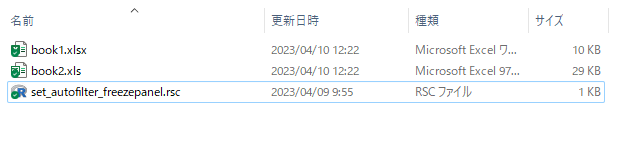
\includegraphics[width=0.8\textwidth,height=\textheight]{img/set_autofilter_freezepanel01.png}\\
\item
  実行前のエクセルのファイル\\
  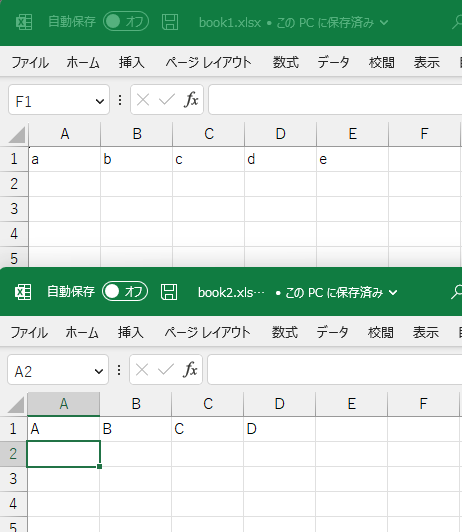
\includegraphics[width=0.4\textwidth,height=\textheight]{img/set_autofilter_freezepanel02.png}\\
\item
  スクリプトの関連付けを参考にして,「.rsc」を「Rscript.exe」に関連付けする(Windowsの場合).Macの場合は,Mac - 拡張子に関連付けられているアプリを変更する方法などを参考にしてほしい.\\
\item
  set\_autofilter\_freezepanel.rsc をダブルクリックして実行すると,黒い画面が表示されてプログラムが実行される.\\
  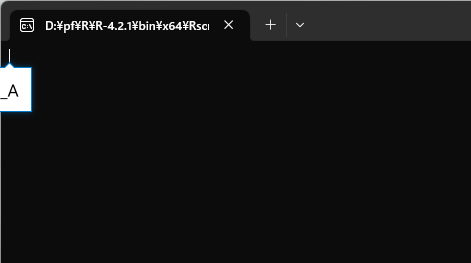
\includegraphics[width=0.4\textwidth,height=\textheight]{img/set_autofilter_freezepanel03.png}\\
  プログラムが自動的にエクセルのファイルの1行目のA列からZ列までにオートフィルタを設定し,1行目と1列目でウィンドウ枠を固定する.
  複数ファイル・複数シートにも対応している.\\
  なお,初回実行時は,xlsxパケージのダウンロードのため,少し時間がかかるかもしれない.
  2回目以降はファイル数が多すぎなければ,一瞬で処理されるはず.
\end{itemize}

実行後のエクセルのファイル\\
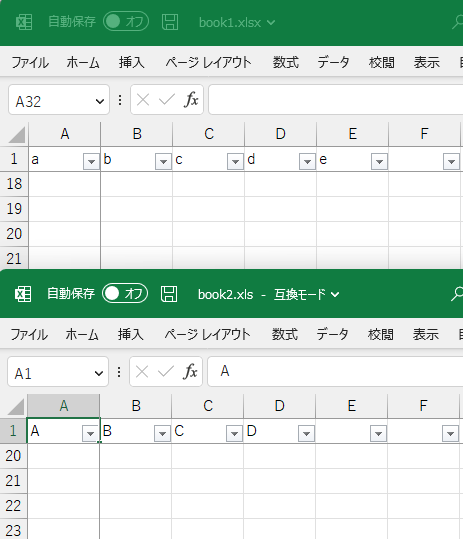
\includegraphics[width=0.4\textwidth,height=\textheight]{img/set_autofilter_freezepanel04.png}

\hypertarget{ux30b9ux30afux30eaux30d7ux30c8ux306eux5185ux5bb9ux8aacux660e}{%
\subsubsection{スクリプトの内容説明}\label{ux30b9ux30afux30eaux30d7ux30c8ux306eux5185ux5bb9ux8aacux660e}}

\begin{Shaded}
\begin{Highlighting}[]
  \CommentTok{\# Package, 準備}
\ControlFlowTok{if}\NormalTok{(}\SpecialCharTok{!} \StringTok{"xlsx"} \SpecialCharTok{\%in\%} \FunctionTok{installed.packages}\NormalTok{()[,}\DecValTok{1}\NormalTok{])\{  }\CommentTok{\# xlsxパッケージ有無の確認}
  \CommentTok{\# パッケージが無い場合}
  \FunctionTok{options}\NormalTok{(}\AttributeTok{repos =} \StringTok{"https://cran.ism.ac.jp/"}\NormalTok{) }\CommentTok{\# ミラーサイトの設定}
  \FunctionTok{install.packages}\NormalTok{(}\StringTok{"xlsx"}\NormalTok{)                   }\CommentTok{\# パッケージのインストール}
\NormalTok{\}}

  \CommentTok{\# Functions, 関数}
\NormalTok{set\_auto\_filter }\OtherTok{\textless{}{-}} \ControlFlowTok{function}\NormalTok{(sh)\{}
  \CommentTok{\# A1からZ1までにオートフィルタを設定}
  \CommentTok{\#   もっと多くの列で設定したければ,"A1:Z1"のところを修正する}
\NormalTok{  xlsx}\SpecialCharTok{::}\FunctionTok{addAutoFilter}\NormalTok{(sh, }\StringTok{"A1:Z1"}\NormalTok{)}
\NormalTok{\}}
\NormalTok{set\_freeze\_panel }\OtherTok{\textless{}{-}} \ControlFlowTok{function}\NormalTok{(sh)\{}
  \CommentTok{\# 1列目と1行目のウィンドウ枠を固定}
  \CommentTok{\#   固定する場所の変更方法}
  \CommentTok{\#     2行目までを固定したい場合は,引数の2つ目と4つ目を,3にする}
  \CommentTok{\#     3列目までを固定したい場合は,引数の3つ目と5つ目を,4にする}
\NormalTok{  xlsx}\SpecialCharTok{::}\FunctionTok{createFreezePane}\NormalTok{(sh, }\DecValTok{2}\NormalTok{, }\DecValTok{2}\NormalTok{, }\DecValTok{2}\NormalTok{, }\DecValTok{2}\NormalTok{)}
\NormalTok{\}}
\NormalTok{set\_af\_fp }\OtherTok{\textless{}{-}} \ControlFlowTok{function}\NormalTok{(file)\{}
\NormalTok{  wb }\OtherTok{\textless{}{-}}\NormalTok{ xlsx}\SpecialCharTok{::}\FunctionTok{loadWorkbook}\NormalTok{(file)   }\CommentTok{\# ワークブックの読み込み}
  \ControlFlowTok{for}\NormalTok{(sh }\ControlFlowTok{in}\NormalTok{ xlsx}\SpecialCharTok{::}\FunctionTok{getSheets}\NormalTok{(wb))\{  }\CommentTok{\# シートの数だけ繰り返し}
    \FunctionTok{set\_auto\_filter}\NormalTok{(sh)            }\CommentTok{\#   オートフィルタの設定}
    \FunctionTok{set\_freeze\_panel}\NormalTok{(sh)           }\CommentTok{\#   ウィンドウ枠の固定}
\NormalTok{  \}}
\NormalTok{  xlsx}\SpecialCharTok{::}\FunctionTok{saveWorkbook}\NormalTok{(wb, file)     }\CommentTok{\# ワークブクの保存}
\NormalTok{\}}

  \CommentTok{\# Main, 本体}
\NormalTok{files }\OtherTok{\textless{}{-}} \FunctionTok{list.files}\NormalTok{(}\AttributeTok{pattern =} \StringTok{"xls"}\NormalTok{) }\CommentTok{\# ".xls"と"xlsx"の一覧取得}
\ControlFlowTok{for}\NormalTok{(file }\ControlFlowTok{in}\NormalTok{ files)\{                  }\CommentTok{\# ファイルの数だけ繰り返し}
  \FunctionTok{set\_af\_fp}\NormalTok{(file)                    }\CommentTok{\# set\_af\_fp()の実行}
\NormalTok{\}}
\end{Highlighting}
\end{Shaded}

\hypertarget{ux305dux306eux4ed6ux306eux64cdux4f5cux672aux4f5cux6210}{%
\subsection{その他の操作(未作成)}\label{ux305dux306eux4ed6ux306eux64cdux4f5cux672aux4f5cux6210}}

\end{document}
